\documentclass[a4paper,ngerman,landscape]{scrartcl}

\usepackage[utf8]{inputenc}

\usepackage[ngerman]{babel}
\usepackage{hyperref}

\usepackage{graphicx}

\usepackage[protrusion=true,expansion=true]{microtype}

\usepackage{lmodern}
\usepackage{tabto}

\setlength\parskip{\medskipamount}
\setlength\parindent{0pt}

\usepackage{geometry}
\geometry{tmargin=0.5cm,bmargin=0.0cm,lmargin=2.5cm,rmargin=2.5cm}

\pagestyle{empty}

\begin{document}

\begin{center}
  \Huge
  Mittwoch, 4. September 2013, 10:00 Uhr, 2004/L1 \\
  \textbf{Ingo Blechschmidt: Konstruktive Mathematik III}
  \vfill
  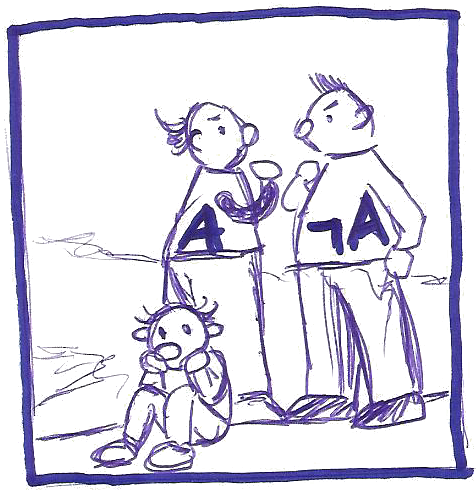
\includegraphics[scale=1.6]{lem}
  \vfill

  \Large
  \begin{minipage}{0.91\textwidth}
    \setlength\parskip{\medskipamount}
    In den bisherigen Vorträgen hatten wir konstruktive Mathematik,
    das ist Mathematik ohne Verwendung des Prinzips vom ausgeschlossenen Dritten,
    kennengelernt, und ihre Beziehung zur klassischen Mathematik diskutiert
    (die tiefer geht als auf den ersten Blick vermutet). Nun wollen wir einen
    Einblick in die Technik des \emph{proof mining} erhalten: Klassische
    Beweise kann man, mehr oder weniger systematisch, nach verstecktem
    konstruktivem Inhalt absuchen, und so teilweise Hilberts Programm
    realisieren. Um das zu illustrieren, werden wir ein einfaches Beispiel aus
    der kommutativen Algebra genauer untersuchen.
  \end{minipage}
\end{center}

\newpage

\begin{center}
  \Huge
  Mittwoch, 4. September 2013, 12:15 Uhr, 2004/L1 \\
  \textbf{Stefan Knoblauch: Knotentheorie I}
  \vfill
  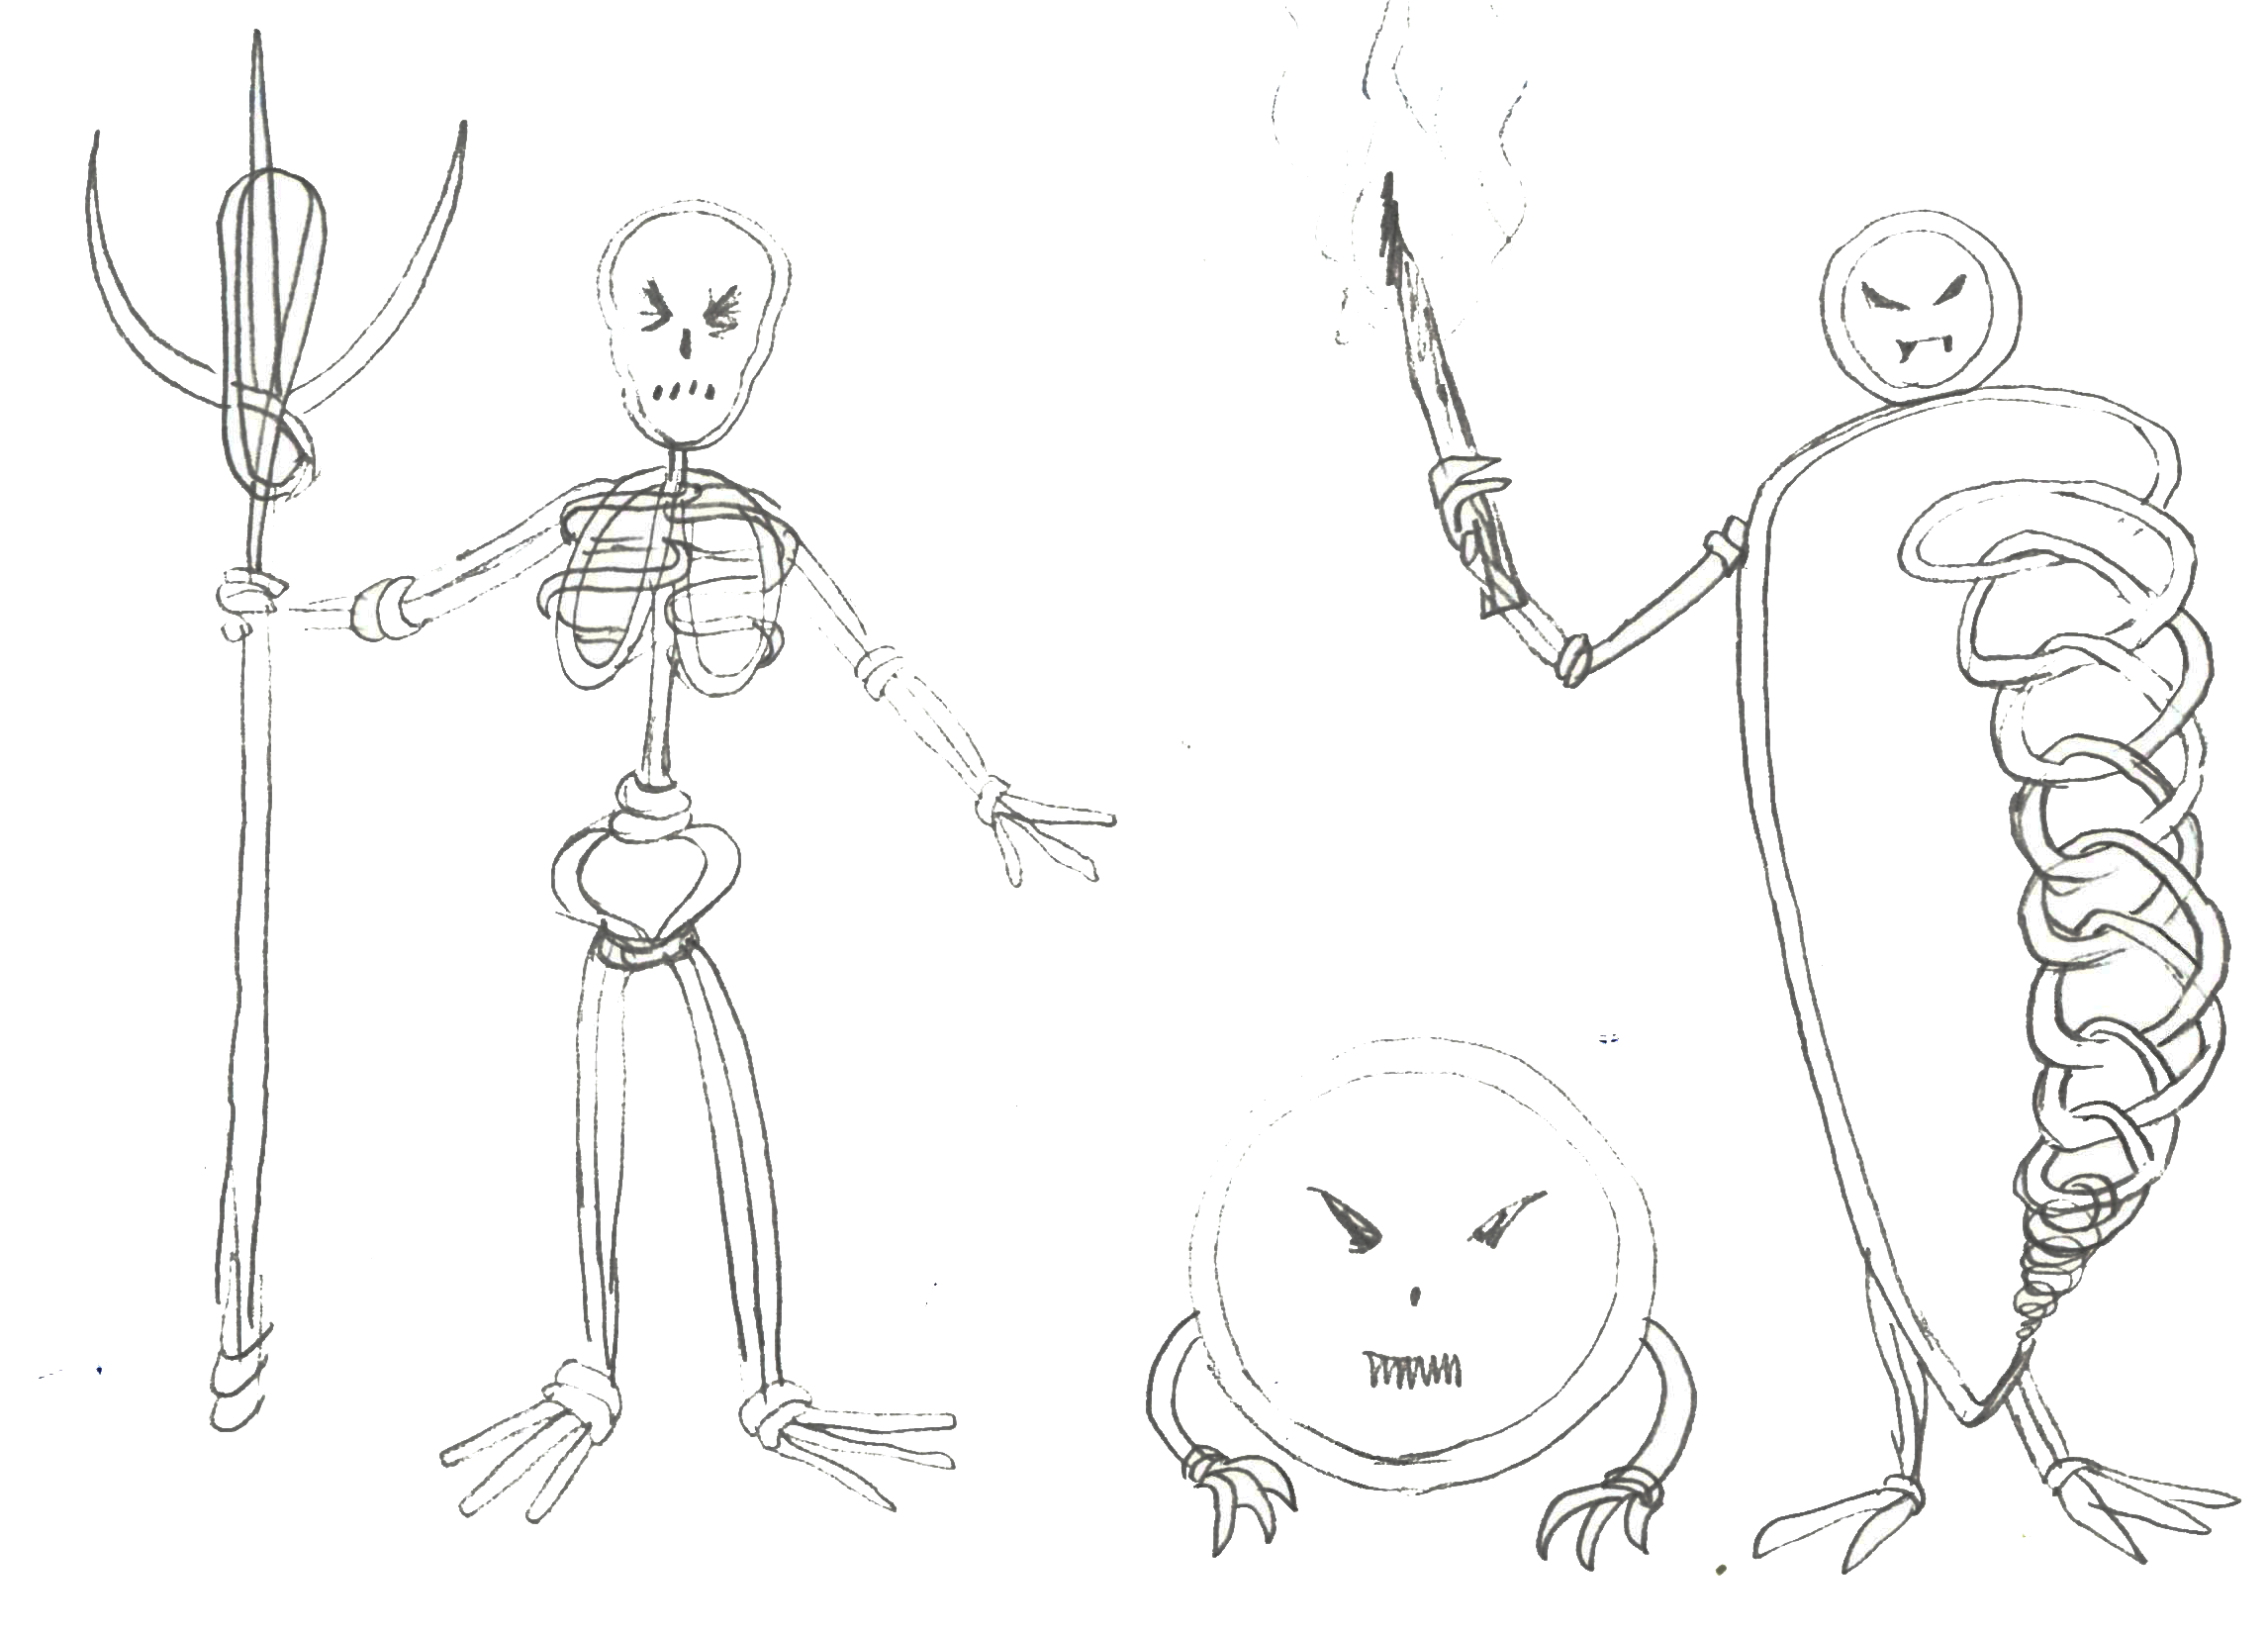
\includegraphics[scale=0.9]{knotenarmee-einfach}
  \vfill

  \Large
  \begin{minipage}{0.91\textwidth}
    \setlength\parskip{\medskipamount}
    Die intuitive Vorstellung geschlossener Knoten kann man mathematisch durch
    Einbettungen der Einheitskreislinie in den dreidimensionalen Raum fassen.
    Dabei beschreiben zwei solche Einbettungen genau dann denselben
    anschaulichen Knoten, wenn sie \emph{umgebungshomotop} zueinander sind; das führt
    auf das Konzept der Fundamentalgruppe. Es gibt auch Einbettungen, die
    keinem anschaulichen Knoten entsprechen: Das sind die sog. \emph{wilden
    Knoten}.

    In diesem ersten Vortrag über Knotentheorie wollen wir all diese Begriffe
    verstehen.
  \end{minipage}
\end{center}
\end{document}
